% !TeX root = ../../main.tex
\subsection{Genome-scale FACS simulation: the effect of dispersion moderation
on the calibration--power tradeoff}

To isolate the FACS design and estimation questions from the
candidate-selected Waterbear validation set, we used CRISPulator 0.5.1
\citep{nagy2017crispulator} to simulate CRISPR knockout screens with known
gene effects at genome scale.  Each of three prespecified seeds generated
10,000 genes, five guides per gene, and four independent screen replicates,
for 50,000 guides per screen.  Twenty percent of genes changed the latent
phenotype and 5\% were explicit negative controls.  The stress-test setting
used phenotype noise $\sigma=2$, 50 sorted cells per guide, and 50 reads per
guide per sample.  Multiplicity of infection was 0.20 in the main analysis
and 0.30 in the supplementary analysis: 0.20 is the operating point at which
the single-integration approximation shared by all of these guide-level
models is most defensible, and 0.30 stresses it.

Each replicate produced a low 0--25\% tail, a high 75--100\% tail, and an
unsorted 0--100\% bulk sample.  The two tails were assigned the conditional
standard-normal locations $-1.271$ and $1.271$; bulk was assigned zero.
Replicate indicators were included in every fit.  We compared this
three-sample fit with the two-tail ablation.  Importantly, ``three sample''
does not mean three independent bins: the bulk sample contains the cell
populations from both tails and costs 50\% more sequencing than the tail-only
design.

Two BARCS gene statistics are carried here.  BARCS-ST
(\texttt{BARCS-original}) is the historical calibrated signed-$z$ statistic.
BARCS-MOD (\texttt{BARCS-moderated}) reuses the same guide fits after
guide-dispersion moderation, which shrinks each guide's variance inflation
toward a library-wide trend before the same signed-$z$ aggregation.  At
genome scale the moderation prior is estimated from 50,000 guides and is
correspondingly sharp: the fitted prior degrees of freedom were 42.7--45.8
against the seven residual degrees of freedom the design itself supplies.

The comparators are the two CRISPR-specific gene callers, MAGeCK-MLE and
CRISPhieRmix \citep{daley2018crisphiermix}, because that is the choice a
screen analyst faces.  They reach the gene level by different routes:
MAGeCK-MLE fits the same design matrix and permutes for its gene FDR, whereas
CRISPhieRmix fits a hierarchical mixture over the guides within a gene, using
the negative-control guides as its empirical null.  It takes guide-level
log$_2$ fold changes, supplied here by a DESeq2 Wald fit of the same design as
its documentation specifies, so DESeq2 enters as a preprocessing step and is
not itself scored.  CRISPhieRmix is run with its bimodal alternative, since
this screen moves the phenotype in both directions and the one-sided default
would score only one of them.

\begin{table}[ht]
\centering
\caption{Genome-scale CRISPulator FACS benchmark at MOI 0.20, 10,000 genes
and 50,000 guides, over three fixed simulation seeds (mean $\pm$ standard
deviation).  All methods are scored on the genes every method returned a
finite result for (9,475--9,517 per run); MAGeCK-MLE omits negative-control
genes from its gene summary once their sgRNAs are declared and CRISPhieRmix
consumes them as its null, so the common set excludes them.  Recall counts
active genes called at gene FDR 0.10 with the
correct direction.  FDP is the realized fraction of inactive genes among
calls; the nominal target is 0.10.  Column maxima for ranking, effect
recovery, recall, and F1 are highlighted.}
\label{tab:crispulator}
\small
\setlength{\tabcolsep}{3pt}
\resizebox{\textwidth}{!}{%
\begin{tabular}{llrrrrrr}
\toprule
Method & Samples & AUROC & Avg.\ precision & Effect $\rho_s$ &
Directional recall & FDP & F1\\
\midrule
\methodswatch{barcsblue} BARCS-ST & Low--bulk--high &
0.947$\pm$.004 & 0.902$\pm$.007 & 0.924$\pm$.004 &
0.716$\pm$.022 & 0.065$\pm$.006 & 0.811$\pm$.012\\
\methodswatch{mageckorange} BARCS-MOD & Low--bulk--high &
0.954$\pm$.003 & 0.919$\pm$.005 & 0.924$\pm$.004 &
0.774$\pm$.014 & 0.066$\pm$.002 &
\textcolor{mageckorange}{\textbf{0.847$\pm$.008}}\\
\methodswatch{naivegray} MAGeCK-MLE & Low--bulk--high &
\textcolor{black}{\textbf{0.957$\pm$.002}} &
\textcolor{black}{\textbf{0.921$\pm$.003}} &
\textcolor{black}{\textbf{0.933$\pm$.002}} &
0.563$\pm$.030 & 0.006$\pm$.002 & 0.718$\pm$.024\\
\methodswatch{chronosgreen} CRISPhieRmix & Low--bulk--high &
0.929$\pm$.004 & 0.867$\pm$.003 & 0.919$\pm$.003 &
0.769$\pm$.025 & 0.197$\pm$.045 & 0.785$\pm$.011\\
\midrule
\methodswatch{barcsblue} BARCS-ST & Low--high &
0.941$\pm$.004 & 0.887$\pm$.008 & 0.923$\pm$.004 &
0.615$\pm$.013 & 0.041$\pm$.001 & 0.749$\pm$.010\\
\methodswatch{mageckorange} BARCS-MOD & Low--high &
0.955$\pm$.003 & 0.920$\pm$.004 & 0.923$\pm$.004 &
0.776$\pm$.012 & 0.063$\pm$.003 & 0.849$\pm$.006\\
\bottomrule
\end{tabular}
}
\end{table}

The two CRISPR-specific comparators fail in opposite directions, and
BARCS-MOD lies between them.  MAGeCK-MLE is the best ranker: it leads AUROC,
average precision, and effect recovery.  CRISPhieRmix is the weakest ranker,
trailing BARCS-MOD by 0.026 AUROC and 0.052 average precision, both intervals
excluding zero.  BARCS-MOD leads F1, and it is the only method here that
combines competitive ranking with a realized FDP below the nominal target.

MAGeCK-MLE converts almost none of its ranking into calls at gene FDR 0.10.
Its realized FDP is 0.006, sixteen times below the 0.10 it was allowed, and
its directional recall is 0.563 against 0.774 for BARCS-MOD.  Paired over the
three seeds its average-precision advantage over BARCS-MOD is 0.0024 (95\%
interval $-0.0029$ to $0.0077$, not resolvable at MOI 0.20), while its F1
deficit is 0.129 ($-0.180$ to $-0.078$).  Its calls are therefore accurate but
highly conservative.  CRISPhieRmix exhibits the converse behavior.  Its
directional recall is statistically indistinguishable from that of BARCS-MOD,
the paired difference being $-0.005$ ($-0.088$ to $+0.078$) and the only such
equivalence in this table, but it attains that recall at realized FDP 0.197
against 0.066, a paired excess of 0.131 (0.018 to 0.245).  Equivalent recall
obtained at three times the error rate is not an equivalent result, and the F1
difference of 0.062 ($0.053$ to $0.071$) quantifies the distinction.

BARCS-MOD therefore attains the operating point that the threshold is intended
to deliver.  It uses most of the permitted false-discovery budget without
exceeding it, 0.066 against the nominal 0.10, and converts this into the
highest F1 among the methods compared.  Neither comparator can be scored on the
negative-control diagnostic, on which BARCS-MOD attains 0.053: MAGeCK-MLE omits negative-control
genes from its gene summary once their sgRNAs are declared, and CRISPhieRmix
consumes them as its empirical null.  That shared omission is also why the
common gene set here is 9,475--9,517 rather than 10,000.

The gain over the historical statistic is unambiguous and is a gain in
ranking rather than a threshold effect: average precision rises from 0.902 to
0.919, a paired difference of 0.017 (0.011 to 0.022), and F1 from 0.811 to
0.847, with realized FDP statistically unchanged.  This is the expected
consequence of estimating the moderation prior from 50,000 guides: a guide
whose own seven residual degrees of freedom understate its variance is
corrected individually, so the negative-control calibration no longer has to
answer those guides with one penalty applied to the whole screen.

Bulk does not supply a new directional contrast.  Across seeds, the
low--bulk--high and tail-only gene effects have mean Spearman correlation
above 0.998.  For the historical statistic its practical contribution is to
the fitted baseline, dispersion, and residual degrees of freedom: mean
directional recall rises from 0.615 to 0.716 and F1 from 0.749 to 0.811, at
50\% more reads.  Moderation largely removes that dependence.  BARCS-MOD
reaches F1 0.849 on the two tails alone against 0.847 with bulk added, so the
information the bulk sample was supplying to the variance model is recovered
more cheaply by borrowing it across the library.  Because the bulk pool
overlaps the tails, its apparent inferential gain may in any case partly
reflect an independence approximation rather than new biological information;
that reading is strengthened by its being replaceable.

\paragraph{Robustness of FDR control across cutoffs.}
The realized-FDP column of Table~\ref{tab:crispulator} is a single point, and
0.10 is in any case looser than a genome-wide screen would use.  We therefore
repeated the calibration check on a log-spaced grid of thirteen cutoffs from
$10^{-6}$ to 0.20 in every run.  The quantity of interest is the ratio of
realized FDP to the cutoff requested: one is exact calibration, below one is
conservative, and above one means the method returns more false discoveries
than it advertised.

\begin{table}[ht]
\centering
\caption{Realized FDP divided by the requested gene-FDR cutoff, MOI 0.20,
means over three seeds on the common gene set; a decade-spaced subset of the
scanned grid is shown.  One is exact calibration and values above one are
violations.  The final column counts the cutoff-by-seed cells, of
$13\times3=39$, in which realized FDP did not exceed the cutoff.}
\label{tab:crispulator-fdr-robust}
\small
\setlength{\tabcolsep}{5pt}
\begin{tabular}{lrrrrrrrr}
\toprule
Method & $10^{-6}$ & $10^{-5}$ & $10^{-4}$ & $10^{-3}$ & 0.01 & 0.05 & 0.10 &
Cells held\\
\midrule
\methodswatch{barcsblue} BARCS-ST &
0.0 & 0.0 & 0.0 & 0.6 & 0.6 & 0.6 & 0.7 & 37/39\\
\methodswatch{mageckorange} BARCS-MOD &
0.0 & 0.0 & 0.0 & 0.4 & 0.7 & 0.6 & 0.7 & 37/39\\
\methodswatch{naivegray} MAGeCK-MLE &
0.0 & 0.0 & 0.0 & 0.0 & 0.1 & 0.1 & 0.1 &
\textcolor{black}{\textbf{39/39}}\\
\methodswatch{chronosgreen} CRISPhieRmix &
0.0 & 0.0 & 0.0 & 0.0 & 1.7 & 2.0 & 2.0 & 22/39\\
\bottomrule
\end{tabular}
\end{table}

CRISPhieRmix overshoots by about twofold wherever it makes enough calls to be
measured, holding 22 of 39 cells.  Its zeros at the strict end do not
indicate calibration: it returns almost nothing there, 0 and 4 genes at
$10^{-6}$ and $10^{-5}$, so no calls exist against which error could be
assessed.  The strict end is precisely the regime relevant to a genome-wide
screen, in which a short and reliable hit list is the objective.  Both BARCS statistics track the requested rate down to
$10^{-4}$ and return no false discoveries at all below it, holding 37 of 39
cells while still calling 276 genes at $10^{-6}$; MAGeCK-MLE holds all 39 but
never uses more than a tenth of the permitted budget.

The exceptions for BARCS should be stated explicitly rather than omitted.  Both
statistics miss 2 of 39 cells, all from one seed (20250725) at the $3\times
10^{-4}$ and $10^{-3}$ cutoffs, and each miss is a single false discovery
against an allowance below one gene.  These are Monte Carlo granularity, not a
systematic failure, and they are the reason the calibration claim in this
paper is stated as a screen average rather than a finite-sample guarantee.  At
MOI 0.30 the same pattern holds, with BARCS-MOD holding 35 of 39 and
CRISPhieRmix 24 of 39.

\paragraph{F1 across cutoffs.}
The same scan reports F1 at every cutoff.  We report it across the grid
rather than at one threshold because a single-threshold F1 compares methods
sitting at different real error rates, and the ordering it produces can depend
on where that threshold falls.

\begin{table}[ht]
\centering
\caption{F1 across requested gene-FDR cutoffs, MOI 0.20, means over three
seeds.  BARCS-MOD leads from $10^{-5}$ upward.  MAGeCK-MLE's constant column
below $10^{-3}$ is a resolution floor rather than performance, and is
quantified below.}
\label{tab:crispulator-f1-cutoffs}
\small
\setlength{\tabcolsep}{6pt}
\begin{tabular}{lrrrrrrr}
\toprule
Method & $10^{-6}$ & $10^{-5}$ & $10^{-4}$ & $10^{-3}$ & 0.01 & 0.05 & 0.10\\
\midrule
\methodswatch{barcsblue} BARCS-ST &
0.046 & 0.126 & 0.262 & 0.456 & 0.653 & 0.774 & 0.811\\
\methodswatch{mageckorange} BARCS-MOD &
0.248 & \textcolor{mageckorange}{\textbf{0.354}} &
\textcolor{mageckorange}{\textbf{0.479}} &
\textcolor{mageckorange}{\textbf{0.607}} &
\textcolor{mageckorange}{\textbf{0.748}} &
\textcolor{mageckorange}{\textbf{0.827}} &
\textcolor{mageckorange}{\textbf{0.847}}\\
\methodswatch{naivegray} MAGeCK-MLE &
\textcolor{black}{\textbf{0.306}} & 0.306 & 0.306 & 0.306 & 0.403 & 0.622 &
0.718\\
\methodswatch{chronosgreen} CRISPhieRmix &
0.000 & 0.004 & 0.080 & 0.321 & 0.634 & 0.780 & 0.785\\
\bottomrule
\end{tabular}
\end{table}

Restricted to CRISPR-specific callers the ordering is stable: BARCS-MOD leads
F1 at every cutoff from $10^{-5}$ to 0.10.  The single exception is
$10^{-6}$, where MAGeCK-MLE's 0.306 exceeds BARCS-MOD's 0.248, and that is not
a result---its call count is identically 358 from $10^{-6}$ to $3\times
10^{-3}$, so the entry is a quantization artifact rather than a measurement.
CRISPhieRmix is the mirror image: it collapses at the strict end, to F1 0.000
and 0.004 at $10^{-6}$ and $10^{-5}$, because it has essentially stopped
calling.

That stability requires careful statement, because it is a consequence of the
comparison set.  A fixed requested cutoff does not place different methods at
the same real error rate, and a method that overshoots its cutoff will look
strong on F1 for that reason alone.  Matching on realized FDP removes the
confound:

\begin{table}[ht]
\centering
\caption{F1 at matched realized FDP, MOI 0.20, interpolated within each run
before averaging over the three seeds.  A dash marks a target outside the
realized-FDP range a method attains on the scanned grid: MAGeCK-MLE never
reaches a realized FDP of 0.05.  Spread is the range across all four methods.}
\label{tab:crispulator-matched-fdp}
\small
\setlength{\tabcolsep}{6pt}
\begin{tabular}{lrrrrrrr}
\toprule
Method & 0.001 & 0.002 & 0.005 & 0.01 & 0.02 & 0.05 & 0.10\\
\midrule
\methodswatch{barcsblue} BARCS-ST &
0.491 & 0.529 & 0.631 & 0.678 & 0.738 & 0.795 & 0.819\\
\methodswatch{mageckorange} BARCS-MOD &
\textcolor{mageckorange}{\textbf{0.640}} &
\textcolor{mageckorange}{\textbf{0.677}} &
\textcolor{mageckorange}{\textbf{0.724}} &
\textcolor{mageckorange}{\textbf{0.764}} &
\textcolor{mageckorange}{\textbf{0.808}} &
\textcolor{mageckorange}{\textbf{0.838}} &
\textcolor{mageckorange}{\textbf{0.847}}\\
\methodswatch{naivegray} MAGeCK-MLE &
0.469 & 0.509 & 0.666 & 0.739 & 0.789 & --- & ---\\
\methodswatch{chronosgreen} CRISPhieRmix &
0.372 & 0.415 & 0.488 & 0.553 & 0.640 & 0.725 & 0.775\\
\midrule
Spread & 0.268 & 0.262 & 0.236 & 0.211 & 0.168 & 0.113 & 0.072\\
\bottomrule
\end{tabular}
\end{table}

BARCS-MOD leads at every matched realized FDP, from 0.640 against 0.372--0.491
at a matched 0.001 to 0.847 against 0.775--0.819 at a matched 0.10.  This is a
stronger statement than the nominal-cutoff table supports on its own, because
it holds the error rate fixed: at the same realized error rate, moderated
BARCS recovers more genes than either CRISPR-specific comparator.  The lead
narrows as the error budget grows, from 0.268 of spread at 0.001 to 0.072 at
0.10, as expected: the methods have less scope to differ when all of them are
permitted a higher error rate.

Two qualifications limit the scope of this comparison.  MAGeCK-MLE's entries in the two
strictest columns rest on its quantized FDR and should be read as indicative;
and it has no entry at all at matched 0.05 or 0.10 because it never becomes
that liberal, so its absence there is conservatism rather than failure.  The
improvement of BARCS-MOD over BARCS-ST is the cleanest comparison in the
table, being larger at every matched error rate, which makes moderation a
genuine gain within the BARCS family rather than a threshold artifact.

\paragraph{MAGeCK-MLE cannot be compared at strict cutoffs, and more
permutations do not fix it.}
MAGeCK-MLE's call count is constant across several orders of magnitude of
requested FDR, which is a property of its inference rather than of the data.
Its gene $p$-value is a permutation tail probability estimated from
$\text{genes}\times\text{rounds}$ draws, so it is quantized in steps of about
$1/(\text{genes}\times\text{rounds})$, and any gene whose statistic exceeds
every permuted value is reported with $p$ exactly zero.  Such genes are called
at any cutoff however strict, which is what produces the plateau.

Refitting one realization at ten rounds instead of one confirms the mechanism
and shows that it is not a settings artifact that can simply be corrected.
The smallest positive $p$-value falls from $2\times10^{-4}$ to
$2\times10^{-5}$, matching the predicted $1/(9475\times\text{rounds})$ to
within the two-sided factor, and the number of genes at $p=0$ falls from 186
to 66.  But the plateau does not disappear: with ten rounds the call count is
still flat, at 66 genes from $10^{-6}$ through $10^{-3}$, and the F1 over that
range \emph{falls} from 0.174 to 0.065 because fewer genes reach $p=0$.  More
permutation moves the plateau down rather than removing it, so MAGeCK-MLE's
strict-cutoff position is set by a computational budget rather than by the
screen.

Resolving a gene FDR of $10^{-6}$ at this library size would need on the order
of $10^{6}/9475\approx110$ rounds, roughly fourteen hours per realization at
the throughput measured here.  We therefore read MAGeCK-MLE's curve below a
requested $10^{-2}$ as not resolvable rather than as a performance result, and
exclude it from the strict-regime comparison; the same caution applies to any
permutation-based gene FDR used at genome scale.  This is measured in
\repofile{examples/crispulator_facs_mageck_permutation_resolution.R}.

\begin{figure}[!t]
\centering
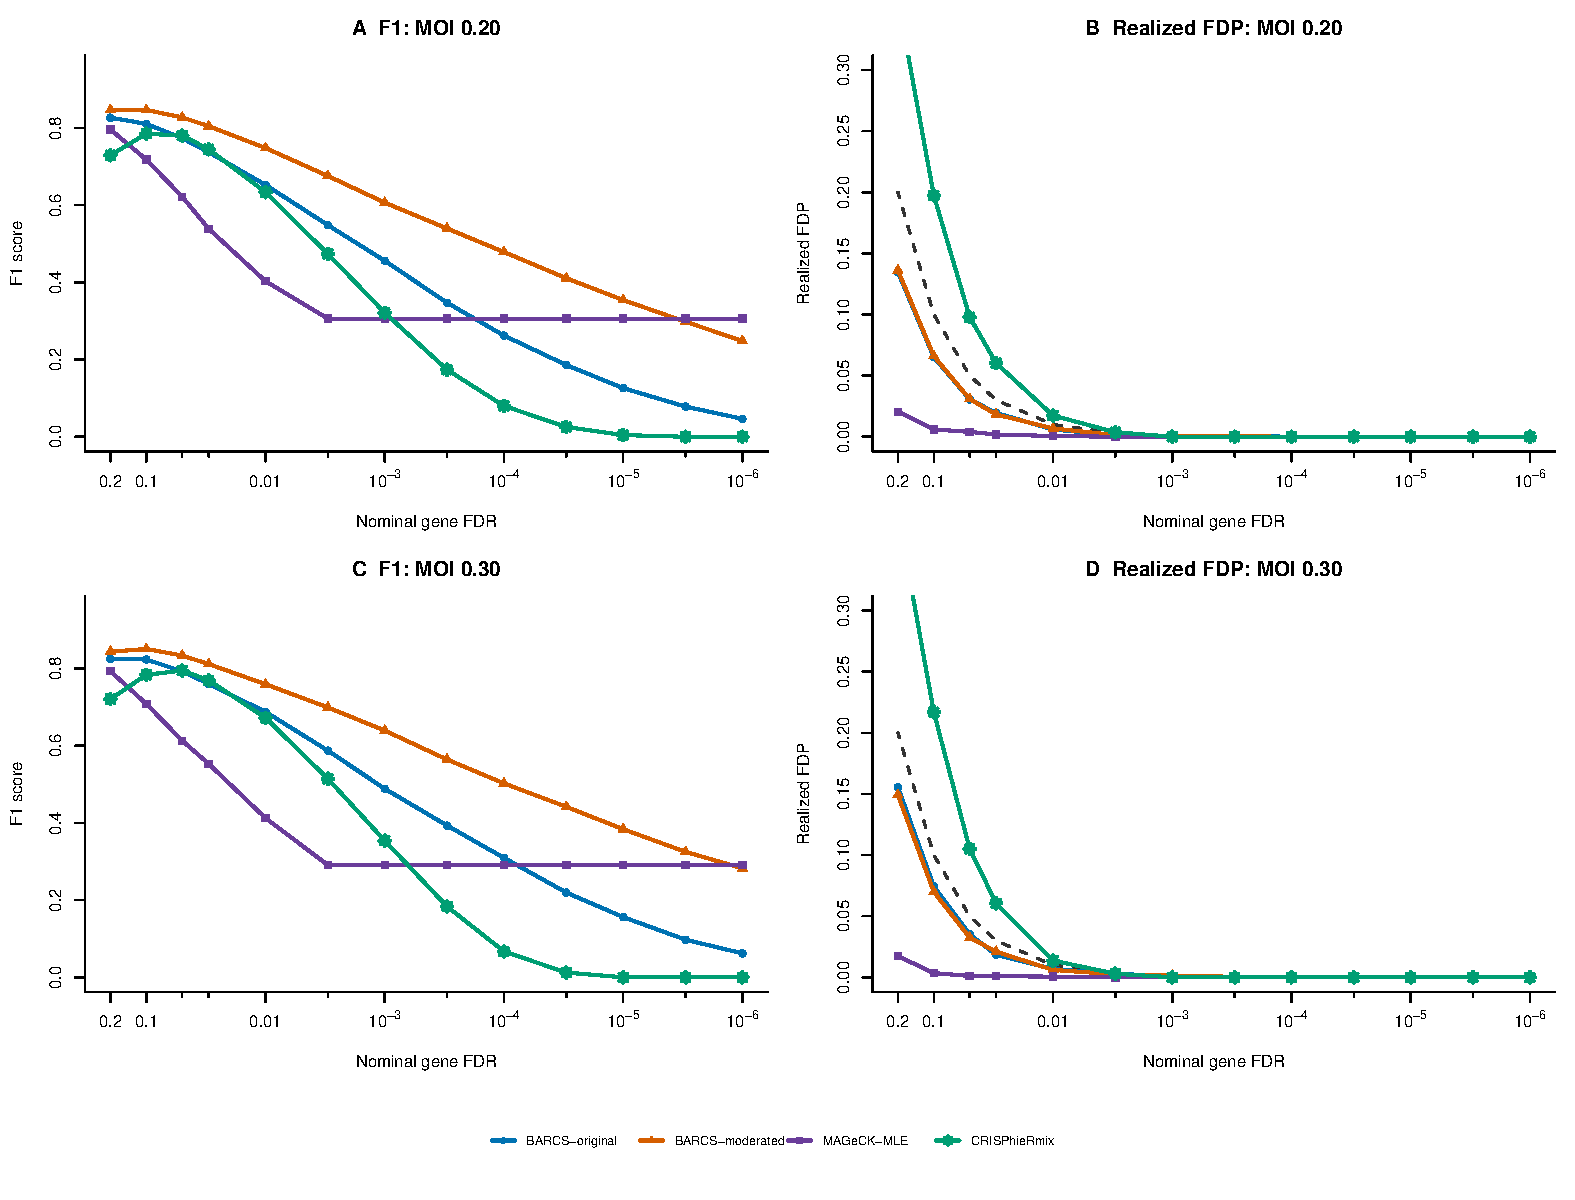
\includegraphics[width=\textwidth]{figures/crispulator_facs_moi_10k_f1_by_fdr.pdf}
\caption{Calibration and F1 across gene-FDR cutoffs in the genome-scale
simulation, means over three seeds on the common gene set.
(A) F1 and (B) realized FDP at MOI 0.20; (C) and (D) the same at MOI 0.30.
The dashed line in the FDP panels is realized equal to nominal, so a method
tracking it reports the error rate it delivers.  Thresholds above 0.10 are a
diagnostic: they show what each method could attain if its threshold were
chosen with knowledge of the truth, which a real screen does not have.}
\label{fig:crispulator-moi10k-fdr}
\end{figure}

At MOI 0.30 every one of these conclusions is reproduced.  BARCS-MOD again leads F1 at
FDP 0.070, CRISPhieRmix again attains its recall at FDP 0.217, and MAGeCK-MLE
again ranks marginally best while calling least, at FDP 0.003 and F1 0.708.
The one difference is that MAGeCK-MLE's average-precision margin over
BARCS-MOD is resolvable at this MOI, 0.0033 (0.0017 to 0.0049).  At the higher
multiplicity CRISPhieRmix marginally exceeds BARCS-MOD on directional recall,
0.785 against 0.784, but at three times the realized error rate, so the
ordering that matters is unchanged.


\paragraph{Supporting 400-gene sensitivity to MOI, guide quality, library
size, and replication.}
The remaining simulation analyses in this subsection are the earlier
400-gene grid, retained because they map the parameter boundaries that the
genome-scale benchmark deliberately does not vary, including the
one-replicate boundary.  They predate the moderated statistic and use the
historical BARCS-ST default and the earlier
$\mathrm{MOI}\in\{0.10,0.25,0.40\}$ levels, so they should be read as
boundary mapping rather than as the headline comparison.  We
varied MOI, the high-quality-guide fraction, the number of genes, and the
number of independent screen replicates one at a time, using five paired seeds
at every setting (ten unique settings and 50 simulations in total).  Nine
settings had at least three replicates; the one-replicate setting was a
prespecified diagnostic boundary.  Among the supported settings, in the
primary low--bulk--high comparison,
BARCS-minus-MAGeCK-MLE average precision ranged only from $-0.015$ to $0.022$
and changed sign across settings.  Thus this experiment does not support a
general ranking advantage for BARCS.  Its more consistent strength was
directional recovery at the prespecified FDR threshold: the directional-recall
difference was positive in seven of nine settings and ranged from $-0.018$ to
$0.136$, while the F1 difference ranged from $-0.022$ to $0.080$.

The largest directional-recall differences occurred at MOI 0.10
($+0.107$) and a high-quality-guide fraction of 0.75 ($+0.119$).  At MOI
0.40, however, MAGeCK-MLE led directional recall by $0.018$ and F1 by
$0.022$; with only 60\% high-quality guides, the methods were nearly tied on
directional recall and MAGeCK-MLE led F1 by $0.005$.  Across 100, 400, and
1,000 genes, BARCS directional-recall differences were $+0.081$, $+0.047$,
and $+0.064$, respectively, whereas average-precision differences again
remained small.  The 100-gene setting also produced realized FDP above 0.10
for both methods (0.181 for BARCS and 0.147 for MAGeCK-MLE), warning that five
small-library replicates do not establish finite-sample FDR control.  These
results sharpen the claim: BARCS can improve directionally correct thresholded
recovery under some noisy or low-MOI conditions, but neither method dominates
every metric or simulation regime.

Replication changed that comparison.  With three replicates, BARCS exceeded
MAGeCK-MLE in directional recall by 0.136 and F1 by 0.080; with four
replicates the differences were 0.047 and 0.011.  At six replicates the signs
reversed slightly, to $-0.012$ for directional recall and $-0.014$ for F1.
The practical interpretation is not that fewer replicates are desirable:
average precision, recall, and F1 increased for both methods as replication
increased.  Rather, BARCS's relative sensitivity is largest in the
low-replication regime, whereas MAGeCK-MLE becomes comparable when information is
abundant.

One replicate crossed from low information into non-confirmatory inference.
Ordinary BARCS retained higher average precision than MAGeCK-MLE, 0.633 versus
0.548, but made no discoveries at gene FDR 0.10 across the five seeds;
MAGeCK-MLE's mean directional recall was only 0.014.  The new BARCS-GC
guide-consistency statistic increased average precision to 0.670,
directional recall to 0.145, and F1 to 0.245.  It made 58 calls across the
five simulations (3--19 per seed), all of which were active genes under the
simulated truth, for mean realized FDP 0.  The fitted empirical-null scales
were 2.19--2.60, showing why an unscaled Wald reference would have been
anti-conservative.

This improvement is useful but deliberately narrow.  BARCS-GC asks whether
independently designed guides give concordant signed effects and assumes that
fewer than half of genes are active; it does not create biological replication.
Its empirical-null calls are therefore hypothesis-generating, not
confirmatory.  We recommend an independent screen for confirmation even when
BARCS-GC is used to prioritize genes from an otherwise irreplaceable $R=1$
experiment.



\noindent\begin{minipage}{\textwidth}
At the four-replicate baseline, mean core fitting times were 0.35 seconds for
BARCS and 4.34 seconds for MAGeCK-MLE.  These measurements exclude
simulation, file input/output, and guide-to-gene aggregation; they show that
the broader comparison is computationally practical but should not be read as
an end-to-end software benchmark.
\end{minipage}

\clearpage
